\subsubsection{Neural networks}
\label{sub:neural_networks}

The origins of the term \textit{\gls{nn}} lie in the attempt to find mathematical representations of information processing in biological systems such as the human brain where the sheets of tissue may be understood as vectors of neurons. While assuming biological realism in pattern recognition is impractical and imposes too many unnecessary constraints, \gls{nn}s have proven to be capable of solving complex problems. The main reason for this is being able to get rid of the task of feature selection. Before the rise of \gls{nn}s, scientists and researchers had to complete the laborious task of coming up with good features to solve learning problems. Their structure enables the learning of useful representations of the input data by creating complex data representations through the combination of simpler ones. The most simple and also most successful model of this type is known as the (three layered) \textbf{\gls{mlp}} (in the following simply denoted as \gls{nn}), which will now shortly be presented. Later on (subsection~\ref{sub:neural_language_models}), more complex neural network architectures will be presented especially under the aspect of their aptitude for \gls{nlp} tasks.

A typical linear model for regression or classification is based on linear combinations of fixed nonlinear basis functions $ \phi_j (\boldsymbol{x}) $ and takes on the form
\begin{equation}
	\label{eq:lin_comb_of_nonlinear_basis_func}
	y(\boldsymbol{x}, \boldsymbol{w}) = f \left( \sum_{j=1}^{M} w_j \phi_j (\boldsymbol{x}) \right)
\end{equation}
where $ f(\cdot) $ is a nonlinear activation function. How \gls{nn}s extend this model is by making the basis functions $ \phi_j(\boldsymbol{x}) $ depend on the parameters and then allow these parameters to be adjusted, along with the coefficients $  \{w_j\} $ during training. This gives us a basic \gls{nn} that can be described as a series of functional transformations. First, $ M $ linear combinations of the input variables $ x_1, \dots, x_D $ in the form
\begin{equation}
	a_j = \sum_{i=1}^{D} w_{ji}^{(1)} x_i + w_{j0}^{(1)}
\end{equation}
need to be constructed where $ j = 1, \dots, M $ with $ M $ being the number of hidden neurons, $ D $ denotes the input dimension and the superscript $ (1) $ indicates that the corresponding parameters are in the first `layer' of the network. The model parameters $ w_{ji}^{(1)} $ are called \textit{weights} and the parameters $ w_{j0} $ are called \textit{biases}. The term $ a_j $ is known as an \textit{activation}. Each activation is then transformed using a differentiable, nonlinear \textit{activation function} $ h (\cdot) $ to give the final output of a neuron:
\begin{equation}
	z_j = h(a_j)
\end{equation}
These quantities are called the \textit{hidden units}. The introduction of non-linearity into the network through these activation functions is a key factor in the success of \gls{nn}s as only using linear activation functions would allow for a creation of an equivalent network without hidden units. This is due to the fact that the composition of successive linear transformations is itself a linear transformation~\footnote{\url{http://www.math.lsa.umich.edu/~kesmith/217worksheet2-3ALT1.pdf}}. As for the implementation of these activation functions there exist different variants that will be listed and explained in the paragraph '\nameref{par:activation_function}'. Following equation~\ref{eq:lin_comb_of_nonlinear_basis_func}, these values are again linearly combined to give \textit{output unit activations}
\begin{equation}
	\label{eq:output_unit_activation}
	a_k = \sum_{j=1}^{M} w_{kj}^{(2)} z_j + w_{k0}^{(2)}
\end{equation}
where $ k = 1, \dots, K $ and $ K $ is the total number of outputs. Equation~\ref{eq:output_unit_activation} represents the second layer of the network. Finally, the output unit activations are transformed using an appropriate activation function to give a set of network ouputs $ y_k $. \\
Now, we can combine these various stages to give the overall network function that takes the form
\begin{equation}
	y_k(\boldsymbol{x}, \boldsymbol{w}) = f \left( \sum_{j=1}^{M} w_{kj}^{(2)} h \left( \frac{1}{2} \right) + w_{k0}^{(2)} \right)
\end{equation}
Thus the neural network model is simply a nonlinear function from a set of input variables $ \{x_i\} $ to a set of output variables $ \{y_k\} $ controlled by a vector $ w $ of adjustable parameters.

Figure~\ref{fig:neural_network_architecture} shows the main components of the \gls{mlp}. The input, hidden, and output variables, or units, are represented by nodes, and the weight parameters, or simply \textit{weights}, are represented by links between the nodes. Additionally, bias parameters, or simply \textit{biases}, are denoted by links coming from additional input and hidden variables $ x_0 $ and $ z_0 $. The arrows demonstrate the direction of information flow through the network during forward propagation.
\begin{figure}
	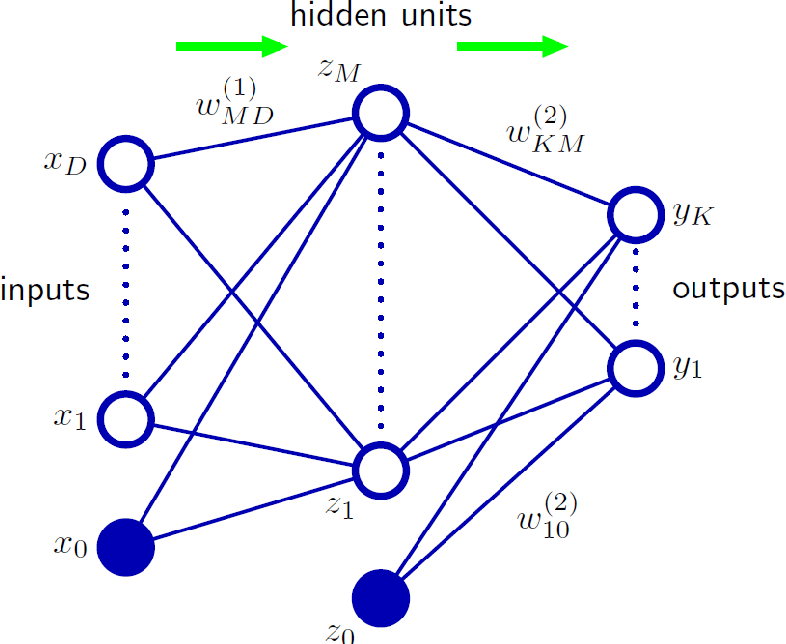
\includegraphics[height=8cm]{img/neural_network_structure}
	\caption{Neural network architecture}
	\label{fig:neural_network_architecture}
\end{figure}

\paragraph{Training process}\label{par:training_process}
The actual tuning of the network's weights are not determined exactly but are usually initialized randomly and iteratively optimized using training data via \textbf{forward propagation}. As this falls into the category of supervised learning, the desired outputs for the training inputs are known and thus a \textbf{cost} or \textbf{loss} function can be used to assess the discrepancy between prediction and ground truth. The calculated error can be used to determine the necessary updates on the weights to improve the predictions in a process called \textbf{backpropagation}. These steps will now be explained individually and in detail.

\paragraph{Activation function}\label{par:activation_function}
In analogy to our biological neurons, artificial neurons can fire a signal depending on the provided input to communicate with the following neurons (or in biology: with the neurotransmitters through electrical impulses). The decision whether a neuron fires or not lies with the activation function. After a single neuron calculates a weighted sum of its input and adds a bias to it, the value of the calculation can be anything from $ -\infty $ to $ +\infty $. As the neuron does not know the bounds of the value it uses an activation function to determine whether it should fire a signal or not.
The easiest option would be to just implement a threshold that fires if $ y > 0 $ and else does not. This, however, poses a problem when dealing with for example multi-classification. In a setting where we have 10 classes and have 2 neurons firing we can not safely say which class the model is more confident on. It would be more helpful to have instead an output of `60\%' or `90\%' activation. A linear function would also not be suited, because of the aforementioned possibility that many linear layers can be replaced by a single layer. That is why most \gls{nn}s nowadays use well-known and established activation functions in their architectures. One of the oldest but still widely used activations is the \textbf{sigmoid function} (in the form of the logistic function)
\begin{equation}
	S(x) = \frac{1}{1+e^{-x}} = \frac {e^{x}}{e^{x}+1}
\end{equation}
The sigmoid function is nonlinear and has no binary activations. Furthermore, it has a smooth gradient which means that the output does not jump in big value ranges. Sigmoids are especially suited for classification tasks, as they tend to bring activations to either `side' of the curve allowing for clear distinctions on prediction. Nonetheless, sigmoids also have a downside: Towards the edges of the domain, the slope on the $ y $-values increases (decreases) less and less which in turn also makes the gradient smaller. This poses a problem as the gradient amongst other things dictates the learning progress of the neural network - and a non-existent gradient also means that there is no learning progress (this problem is typically referred to as \textit{vanishing gradient}). Another frequently mentioned activation function is the \textbf{hyperbolic tangent}
\begin{equation}
	\tanh(x) = \frac{\sinh(x)}{\cosh(x)} = \frac{e^{x}-e^{-x}}{e^{x}+e^{-x}} = \frac{e^{2x}-1}{e^{2x}+1}
\end{equation}
which is basically a scaled sigmoid function. The $ tanh $ function was introduced in order to provide a stronger gradient than sigmoid (for steeper derivatives). Whether sigmoid or tanh activation functions should be chosen depends on the nature of the problem. The sigmoid activation function saturates at zero and one while tanh saturates at plus and minus one. So if the activity in the network during training is close to zero then the gradient for the sigmoid activation function may go to zero. However, the activation function that has had by far the most impact in the world of \gls{ml} and especially deep learning is the \textbf{\gls{relu}}
\begin{equation}
	f(x) = x^{+} = \max(0,x)
\end{equation}
simply because of its non-saturation gradient, which greatly accelerates the convergence of stochastic gradient descent compared to the other two functions~\footcite{10.1145/3065386}. Another useful property of the \gls{relu} function is that it does not need any expensive operations (e.g. exponentials) to be computed, but can simply be implemented by thresholding a matrix of activations at zero.
\begin{figure}
	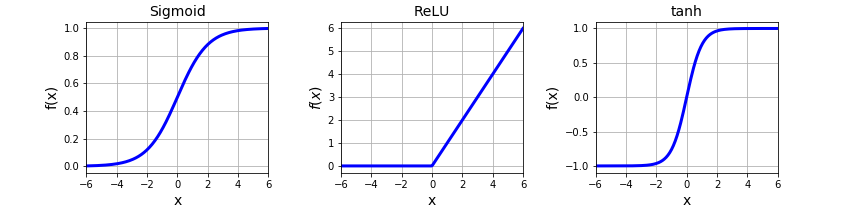
\includegraphics[height=4cm]{img/activation_functions}
	\caption{Different activation functions}
	\label{fig:different_activation_functions}
\end{figure}

\paragraph{Cost function}\label{par:cost_function}
For a neural network to know how and when to update its parameters it needs to know what the underlying optimization problem is that it is facing. This is posed by the so-called \textit{cost function}, or \textit{loss function}, which compares the prediction of the model with the desired value and returns a metric of distance. The gradient at the given input values determines the updates that the neural network will perform on its weights and biases. In the following, two of the most prominent loss functions will be presented and explained. Here, $ y $ denotes the true solution and $ \widetilde{y} $ denotes the prediction as a function $ h $ with parameters $ \theta $ of the input $ x $ of the model. The general equation of a cost function represents the sum of the errors multiplied across the whole batch:
\begin{equation}
	J(\theta) = \frac{1}{\alpha} \sum_{i=1}^{n} \text{C} (h_{\theta} (y^{(i)}), \widetilde{y}^{(i)})
\end{equation}
A simple implementation of the cost function is the \textbf{\gls{mse}} loss, which has analogies to many fields such as mechanical engineering~\footnote{\url{https://projecteuclid.org/download/pdf_1/euclid.bbms/1203692451}}. Here, the square of the difference between prediction and truth is squared, summed up and then divided by the length of the batch.
\begin{equation}
	\frac{1}{N} \sum_{i=1}^{N} \left( y_i - \widetilde{y_i} \right)^2
\end{equation}
One of the standard functions when it comes to classification is the cross-entropy loss function that calculates on step $ t $ the cross-entropy between predicted probability distribution $ \hat{y}^{(t)} $, and the truth $ y^{(t)} $
\begin{equation}
	J^{(t)}(\theta) = \text{CE}(\boldsymbol{y}^{(t)}, \hat{\boldsymbol{y}}^{(t)}) = - \sum_{w \in V} \boldsymbol{y}_w^{(t)} \ \text{log} \ \hat{\boldsymbol{y}}_w^{(t)} = - \text{log} \ \hat{\boldsymbol{y}}_{\boldsymbol{x}_{t+1}}^{(t)}
\end{equation}
Cross entropy relies on probabilities and not just boolean values for class membership, therefore, it allows more precise performance evaluation. Abstractly, cross entropy between two probability distributions can be interpreted as the expected message-length per datum when a wrong distribution $ q $ is assumed while the data actually follows a distribution $ p $.

\paragraph{Backpropagation}\label{par:backprop}
The process of calculating the activations at each hidden layer and the output layers as well as the resulting loss function is known as \textbf{forward propagation}. Now, to actually update the parameters of the neural network the \textit{contribution} of each parameter to the loss (gradient) needs to be computed and each parameter needs to be updated with gradient descent - this process is called \textbf{backpropagation}. The concept of gradient descent can be illustrated in a two-dimensional setting by plotting the `landscape' of the loss function which one is trying to minimize - here the initial value can be seen as the start position of a `ball' that then starts to roll down until it reaches the bottom, or mathematically: the local minimum (figure~\ref{fig:gradient_descent}). The idea of backpropagation was introduced in the 1970s by Finnish master student Seppo Linnainmaa~\footcite{linnainmaa1970representation}. Here, instead of naively calculating the gradient of each layer separately the partial computations of the gradient for each layer are reused in the computation of the gradient for the previous layer. The backpropagation algorithm is dependent on the following 5 equations:

The partial derivatives of the cost function are calculated by
\begin{equation}
	\label{eq:backprop_one}
	\frac{\delta J}{\delta w_{ij}^{k}} = \delta_j^k o_i^{k-1}
\end{equation}
where for each $ \delta_j^k $ is calculated on the final layer's loss term
\begin{equation}
	\label{eq:backprop_two}
	\delta_1^m = g'_o (a_1^m)(\hat{y}_d - y_d)
\end{equation}
and on the hidden layers' loss terms
\begin{equation}
	\label{eq:backprop_three}
	\delta_j^k = g'(a_j^k) \sum_{l=1}^{r^{k+1}} w_{jl}^{k+1} \delta_l^{k+1}
\end{equation}
Combination of the partial derivatives for each input-output pair are takes places like so
\begin{equation}
	\label{eq:backprop_four}
	\frac{\delta J(X, \theta)}{\delta w_{ij}^k} = \frac{1}{N} \sum_{d=1}^{N} \frac{\delta}{\delta w_{ij}^{k}} \left( \frac{1}{2} (\boldsymbol{\hat{y}_d} - \boldsymbol{y_d})^2 \right) = \frac{1}{N} \sum_{d=1}^{N} \frac{\delta J_d}{\delta w_{ij}^k}
\end{equation}
As for updating the weights, one uses
\begin{equation}
	\label{eq:backprop_five}
	\Delta w_{ij}^{k} = - \alpha \frac{\delta J(X, \theta)}{\delta w_{ij}^{k}}
\end{equation}
In the following the simplest form of backpropagation with simple \textit{gradient descent} will be presented.
\begin{enumerate}
	\item Firstly, the forward propagation for each input-output pair $ \boldsymbol{x_d}, \boldsymbol{y_d} $ has to be computed. The results $ \boldsymbol{\hat{y}_d} $, $ \boldsymbol{a_j^k} $ and $ o_j^k $ for each node $ j $ are then stored in layer $ k $ by proceeding from input layer $ 0 $ to the output layer $ m $.
	\item Secondly, the backward phase for each input-output pair $ \boldsymbol{x_d}, \boldsymbol{y_d} $ is calculated and the results $ \frac{\partial J_d}{\partial w_{ij}^{k}} $ for each weight $ w_{ij}^{k} $ connecting node $ i $ in layer $ k - 1 $ to node $ j $ in the next layer are stored starting now on the last layer $ m $ and continuing until layer $ 1 $. This step can be further split up into 3 sub-steps:
	\begin{enumerate}
		\item The term $ \delta_1^m $ is calculated by using equation~\ref{eq:backprop_two}.
		\item The calculated loss terms for the hidden layers $ \delta_j^k $ are backpropagated starting on layer $ k = m - 1 $ through repetitive usage of equation~\ref{eq:backprop_three}.
		\item Now the partial derivatives of individual loss $ J_d $ \gls{wrt} $ w_{ij}^k $ can be evaluated by using equation~\ref{eq:backprop_one}.
	\end{enumerate}
	\item Now, the entirety of the gradient $ \frac{\delta J(X, \theta)}{\delta w_{ij}^k} $ over the entire set of input-output pairs can be calculated by combining the individual input-output pair gradients in equation~\ref{eq:backprop_four}.
	\item The \textbf{learning rate} $ \alpha $ is used in the final formula to update the weights of the network by subtracting the total gradient $ \frac{\delta J(X, \theta)}{\delta w_{ij}^k} $ multiplied by $ \alpha $ (equation~\ref{eq:backprop_five}).
\end{enumerate}
\bigskip

\begin{figure}
	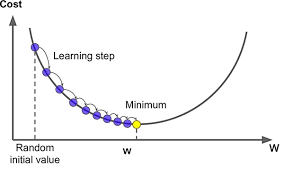
\includegraphics[height=4cm]{img/gradient_descent}
	\caption[Gradient descent on a convex quadratic function]{Gradient descent on a convex quadratic function~\footnote{\url{https://www.topcoder.com/gradient-descent-in-machine-learning/}}}
	\label{fig:gradient_descent}
\end{figure}

There are different variations of the gradient descent optimization, namely batch, stochastic and mini-batch, which will shortly be presented. Each variant differs in how much data is used to compute the gradient of the loss function - which one is best suited depends on the problem. These variations fundamentally are a trade-off between speed and accuracy. \textbf{Batch gradient descent} utilizes the whole dataset, computing the loss of each data point and averaging over the entire set. This takes up a lot of computation, therefore batch gradient descent is considered to be slow. Also using each datapoint many times can cause the algorithm to overfit on the training data. Batch gradient descent works best for functions with very little local minima, as it can easily get stuck in one. In contrast, \textbf{\gls{sgd}} computes the loss and makes the update on a single sample rather than the entire set. This speeds up each gradient step linearly with the size of the data set. Due to noise in the data it can happen though, that the gradient step is performed in the opposite direction of the optimum. \gls{sgd} works best if the function has a lot of local minima since the noise performing the gradient descent on a single data point oftentimes moves the model out of local minimum to maybe a better one. \textbf{Mini-Batch} uses a random subset of the entire dataset and computes the gradient of the loss on that subset. This is a combination of the other two methods so it can reduce the problems they are facing. It takes way less computation performing one step while reducing the noisiness of \gls{sgd}. Choosing the mini-batch size depends on the problem. If possible it should be small enough to still avoid local minima, while being big enough to converge to the global minimum.

